\section{Reducing normal form of a matrix}

In \cref{coloring definition as kernel} we defined the coloring module of a diagram $D$ as the kernel of coloring homomorphism. We might also want to extend this homomorphism to a short exact sequence
\begin{center}
  \begin{tikzcd}
    0\arrow[r] & \ker f\arrow[r, hookrightarrow] & M^s\arrow[r, "f"] & M^s\arrow[r, two heads] & \coker f \arrow[r] & 0
  \end{tikzcd}
\end{center}
and ask what information can be obtained from studying $\coker f$.

In \cref{ex2,,ex3} nontrivial coloring was admissible only in modules $M/\mathfrak{a}$, where $\mathfrak{a}$ is the ideal spanned by a portion of terms that appear on the diagonal of Smith's normal form of $f$. In the same examples, we observe also that $\coker f=R^k\oplus R/\mathfrak{a}$. For the knot $3_1$ it was $\coker f=\Z\oplus \Z_3$, while in the case of knot $4_1$ $\coker f=\Z\oplus \Z_5$.

\begin{proposition}
  Let $f$ be a coloring homomorphism of an oriented diagram $D$. If $\coker f=R/\mathfrak{a}_1\oplus...\oplus R/\mathfrak{a}_k$ then $D$ can be colored with elements from $R/\mathfrak{a}_i$ for $i=1,..., k$.
\end{proposition}

\begin{proof}
  {\color{red}To się powinno sprowadzić do rozwiązywania układu równań przy pomocy macierzy}.
\end{proof}

The coloring homomorphism $f$ of a diagram $D$ carries a lot of information about the knot whose diagram it is. However, $f$ in itself is not a knot invariant. The dimensions of its matrix will change if a new crossing is created, see the following example.

\begin{example}\label{ex4}
  We take knot $3_1$ with additional crossing, $R=\Z[t, t^{-1}]$ and $M=\Z[t, t^{-1}]$ with $\phi$ as in \cref{ex3}. The coloring homomorphism has matrix
  $$
  \begin{pmatrix}
    1-t & t & -1 & 0 \\ 
    t & -1 & 0 & 1-t \\ 
    -1 & 1-t & 0 & t \\ 
    0 & 0 & 1 & -1 
  \end{pmatrix}
  $$
  with normal form
  $$
  \begin{pmatrix}
    -1 & 0 & 0 & 0\\ 
    0 & 1 & 0 & 0 \\ 
    0 & 0 & -t^2+t-1 & 0 \\ 
    0 & 0 & 0 & 0 &
  \end{pmatrix}
  $$
  which after evaluation at $t=-1$ yields
  $$
  \begin{pmatrix}
    -1 & 0 & 0 & 0\\ 
    0 & 1 & 0 & 0 \\ 
    0 & 0 & -3 & 0 \\ 
    0 & 0 & 0 & 0 &
  \end{pmatrix}
  $$
  which differs from matrix obtained in \cref{ex2} by just one trivial.
  \begin{figure}[h]\centering 
    \begin{tikzpicture}
    \begin{knot}[
      clip width=40,
      consider self intersections,
      ignore endpoint intersections=false, 
      flip crossing=2
      ]
      \strand[thick, ->] 
        (90:3) to [out=180, in=-90-30, looseness=2] 
        (-30:3);
      \strand[thick, ->] (-30:3) to [out=60, in=90, looseness=1.5] 
        (200:3.5); 
      \strand[thick, ->] (200:3.5) to[out=-90, in=-30, looseness=1.5] 
        (210:5);
      \strand[thick, ->] (210:5) to[out=180-30, in=180-30, looseness=1.5] 
        (210:3); 
      \strand[thick, ->] (210:3) to[out=-30, in=0, looseness=2]
        (90:3);
    \end{knot}
    \end{tikzpicture}
    \caption{Diagram of knot $3_1$ with additional crossing.\label{trefoil z dodatkowym skrzyzowaniem}}
  \end{figure}
\end{example}

The nontrivial term on the diagonal in \cref{ex4} is the same as in \cref{ex2}. The difference between matrices obtained in those two examples are their dimensions.

\begin{definition}\label{equivalence of matrices definition}
  % Let $f$ be a coloring homomorphism of diagram $D$ with Smith's normal form 
  % $$
  % S=\begin{pmatrix}
  %   a_1 & 0 & 0 & \hdots & 0 & \hdots & 0 \\ 
  %   0 & a_2 & 0\\ 
  %   0 & 0  & \ddots & & \vdots & & \vdots \\ 
  %       & & & a_k \\ 
  %     0 & &\hdots &  & 0 & \hdots & 0 \\ 
  %     \vdots & & & & \vdots & & \vdots\\ 
  %     0 & & \hdots & & 0 & \hdots & 0
  %   \end{pmatrix}
  % $$
  % We will define 
  %
  %
  Let $A$, $B$ be matrices with entries from a PID ring $R$. We will say that they are equivalent ($A\sim B$) if and only if their Smith's normal form has the same nonzero and nonunit terms.
\end{definition}

\begin{example}
  Matrices of coloring homomorphisms over the ring $\Z$ of knot $3_1$ presented in \cref{ex2,,ex4} are both equivalent to a $1\times 1$ matrix $\begin{pmatrix}3\end{pmatrix}$.
\end{example}

\begin{theorem}
  Equivalence class of matrices under relation $\sim$ defined in \cref{equivalence of matrices definition} is a knot invariant.
\end{theorem}







\bigskip

\rule{\textwidth}{1pt}
\bigskip

\begin{example} 
  First, consider the knot $6_1$ with diagram as seen in \cref{fig:6_1:knot}, ring $R=\Z[t, t^{-1}]$ and $M=R$. We calculate that
\begin{figure}[h]\centering
  \begin{tikzpicture}[bgnd/.style={circle, fill=white, draw=white}]
    %\node[opacity=0.2] at (0,0) {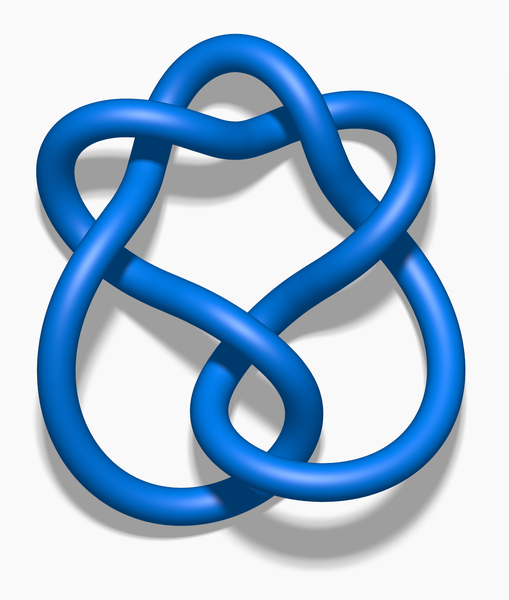
\includegraphics[width=0.7\textwidth]{./rozdzialy/6_1-3d.png}};

    \coordinate (a0) at (0,0);
    \coordinate (a1) at (90:5);
    \coordinate (a2) at (45:3);
    \coordinate (a3) at (-40:4.6);
    \coordinate (a4) at (-120:2.4);
    \coordinate (a5) at (10:0.7);
    \coordinate (a6) at (50:5);
    \coordinate (a7) at (90:3.5);
    \coordinate (a8) at (180-50:5);
    \coordinate (a9) at (170:0.7);
    \coordinate (a10) at (-70:2.4);
    \coordinate (a11) at (220:4.6);
    \coordinate (a12) at (180-45:3);

    %\foreach \i in {0,...,12} \fill (a\i) circle (2pt);

    \begin{knot}[
      clip width=20, 
      flip crossing=1,
      flip crossing=3,
      flip crossing=6
      ]
      \strand[thick, ->] (a1) to[out=0, in=90+45] (a2) to[out=-45, in=40] (a3);
      \strand[thick, ->] (a3) to[out=220, in=-90] (a4) to[out=90, in=200] (a5);
      \strand[thick, ->] (a5) to[out=20, in=-60] (a6);
      \strand[thick, ->] (a6) to[out=150, in=5] (a7);
      \strand[thick, ->] (a7) to[out=170, in=20] (a8);
      \strand[thick, ->] (a8) to[out=240, in=160] (a9);
      \strand[thick, ->] (a9) to[out=-20, in=90] (a10);
      \strand[thick, ->] (a10) to[out=-90, in=-40] (a11);
      \strand[thick, ->] (a11) to[out=140, in=180+45] (a12);
      \strand[thick, ->] (a12) to[out=45, in=180] (a1);
    \end{knot}

    %\node at (80: 5) {$A$};
    %\node at (-40:4) {$B$};
    %\node at (45:5.5) {$C$};
    %\node at (135:5.5) {$D$};
    %\node at (-1.5,0.1) {$E$};
    %\node at (220:4) {$F$};
    %
    %\node[bgnd] at (70:4.7) {$1$};
    %\node[bgnd] at (25:3.9) {$2$};
    %\node[bgnd] at (-90:3) {$3$};
    %\node[bgnd] at (90:0.5) {$4$};
    %\node[bgnd] at (110:4.7) {$5$};
    %\node[bgnd] at (180-25:3.9) {$6$};

    %\draw[dashed] (70: 4) circle (0.4);
    %\draw[dashed] (28: 3.1) circle (0.4);
    %\draw[dashed] (-90:3.5) circle (0.4);
    %\draw[dashed] (-90:0.15) circle (0.4);
    %\draw[dashed] (180-28:3.1) circle (0.4);
    %\draw[dashed] (110:4) circle (0.4);
  \end{tikzpicture}
  \caption{\label{fig:6_1:knot}Diagram of knot $6_1$.}
\end{figure}
$$f=\begin{pmatrix}
  -1 & 0 & 0 & 0 & 0 & 0 \\ 
  0 & -1 & 0 & 0 & 0 & 0 \\ 
  0 & 0 & t & 0 & 0 & 0 \\ 
  0 & 0 & 0 & t & 0 & 0 \\ 
  0 & 0 & 0 & 0 & -2t^{-2}+5t^{-1}-2 & 0 \\ 
  0 & 0 & 0 & 0 & 0 & 0 
\end{pmatrix}$$
which agrees with the Alexander polynomial of $6_1$. Now, the reduced form of $f$ would be 
$$
\begin{pmatrix}
  -2t^{-2}+5t^{-1}-2
\end{pmatrix}
$$
a $1\times 1$ matrix.

There is another knot with Alexander polynomial equal $-2t^{-2}+5t^{-1}-2$: $9_{46}$. Using diagram in \cref{fig:9_46:knot} it can be calculated that  
\begin{figure}[h]\centering
  \begin{tikzpicture}[bgnd/.style={circle, fill=white, draw=white}]
    %\node[opacity=0.2] at (0,0) {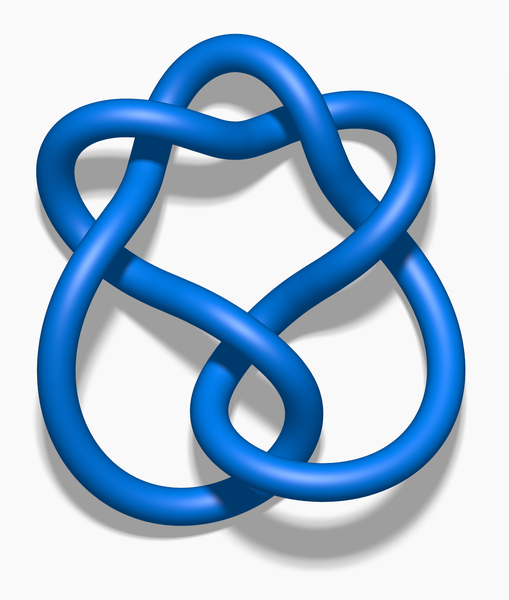
\includegraphics[width=0.7\textwidth]{./rozdzialy/6_1-3d.png}};

    \coordinate (a0) at (0,0);
    \coordinate (a1) at (60:5);
    \coordinate (a2) at (150:3);
    \coordinate (a3) at (-110:2.5);
    \coordinate (a4) at (-60:6);
    \coordinate (a5) at (30:1.5);
    \coordinate (a6) at (200:0.8);
    \coordinate (a7) at (170:5);
    \coordinate (a8) at (120:5);
    \coordinate (a9) at (30:3);
    \coordinate (a10) at (-70:2.5);
    \coordinate (a11) at (180+60:6);
    \coordinate (a12) at (150:1.5);
    \coordinate (a13) at (-20:0.8);
    \coordinate (a14) at (10:5);

    %\foreach \i in {0,...,14} \fill (a\i) circle (2pt);

    \begin{knot}[
      clip width=20, 
      consider self intersections,
      ignore endpoint intersections=false,
      %draft mode=crossings,
      flip crossing=1,
      flip crossing=4,
      flip crossing=7, 
      flip crossing=9
      ]
      \strand[thick, ->] 
        (a1) to [out=180, in=30]
        (a2) to [out=210, in=150]
        (a3);
      \strand[thick, ->]
        (a3) to [out=-30, in=180] 
        (a4) to [out=0, in=-15, looseness=1.5] 
        (a5);
      \strand[thick, ->]
        (a5) to [out=170, in=30] 
        (a6) to [out=220, in=-90] 
        (a7);
      \strand[thick, ->]
        (a7) to [out=90, in=180, looseness=1.3] 
        (a8) to [out=0, in=150] 
        (a9);
      \strand[thick, ->]
        (a9) to [out=-30, in=30]
        (a10) to [out=210, in=0] 
        (a11);
      \strand[thick, ->]
        (a11) to [out=180, in=180+15, looseness=1.5] 
        (a12) to [out=10, in=150]
        (a13);
      \strand[thick, ->]
        (a13) to [out=-40, in=-90]
        (a14) to [out=90, in=0, looseness=1.3]
        (a1);
      \fill[yellow] (-10:3.7) circle (6pt);
    \end{knot}
  \end{tikzpicture}
  \caption{\label{fig:9_46:knot}Diagram of knot $9_{46}$.}
\end{figure}
$$f=\begin{pmatrix}
  1 & 0 & 0 & 0 & 0 & 0 & 0 & 0 & 0 \\ 
  0 & t^{-1} & 0 & 0 & 0 & 0 & 0 & 0 & 0 \\ 
  0 & 0 & t^{-1} & 0 & 0 & 0 & 0 & 0 & 0\\ 
  0 & 0 & 0 & t  & 0 & 0 & 0 & 0 & 0 \\ 
  0 & 0 & 0 & 0 & t  & 0 & 0 & 0 & 0 \\ 
  0 & 0 & 0 & 0 & 0 & t  & 0 & 0 & 0\\ 
  0 & 0 & 0 & 0 & 0 & 0 & 2t-t^2 & 0 & 0 \\ 
  0 & 0 & 0 & 0 & 0 & 0 & 0 & t^{-2}-2t^{-1} & 0\\ 
  0 & 0 & 0 & 0 & 0 & 0 & 0 & 0 & 0
\end{pmatrix}$$
where 
$$\det f= (2t-t^2)(t^{-2}-2t^{-1})=2t^{-1}-5+2t$$
is also the Alexander polynomial. The reduced form of $f$ is
$$
\begin{pmatrix}
  2t-t^2 & 0 \\ 
  0      & t^{-2}-2t^{-1}
\end{pmatrix}
$$
which is significantly different than the one for $6_1$.
\end{example}

{\large\color{red}TO DO: sprawdzić te węzły wyżej za pomocą pow. Seiferta, czy mają różne moduły Alexandera}
